\chapter{Background}\label{ch:chapter2} % For referencing the chapter elsewhere, use \ref{Chapter1}
%
%%----------------------------------------------------------------------------------------
%
To start with, we bring up what is video coding, why it is needed, and
its challenges.
Next we discuss what is deep learning, the history of deep learning and how
it works for vision tasks.
Furthermore, we introduce how we plan to apply deep learning to optimize video
coding tasks and why it should work.
In the end, a survey of related works in video coding and deep learning is given.

%3D Video applications are attracting more interests
%%----------------------------------------------------------------------------------------
%
\section{Video Coding}\label{sec:video-coding}
Video playback is the most straightforward way for human to perceive dynamic
scenes that exist across a time series.
More than half of the neurons in human brain are born to process the visual
information which is supplied by human eyes.
It becomes effortless for human to understand things presented by
the video playback instead of a long paragraph of words.
Videos are made up of consecutive sets of image frames, which in turn
are made up of pixel matrices.
Visual information of a cosmic scale is first stored by various methods
then delivered during a period of video playback.

In 1950s, video tapes were employed to store the videos.
Video tape is able to serve for about eight to twelve years
before the video quality starts to degrade.
In 1970s, laser disc appeared in the US market as an alternative of video tapes.
Start from laser disc, the video storage started its new era in digital world.
In 1990s, DVDs were released after laser disc.
Data is stored in spiralling tracks on the disc.
A laser beam can be utilized to read the data.
In addition, hard drives, flash drives and SD cards were also starting to
become popular in the late 90s.
Nowadays, the cloud storage is very common in daily lives.
It is capable of storing data on the servers which are
accessible from any devices via internet connections.

Although so many formats are available for video storage, they share a common
feature: the more storage you use, the more cost it will be.
Let's take the cloud storage as an example.
Google cloud is one of the most popular cloud services in our daily lives.
It provides cloud storage with a price
of \$0.026 per GB/month~\parencite{RN202}
(this price is observed on 21 Nov 2017, it may change in the future).
If a 4K video with a resolution of 4096*2160,
at 120 frames per second,
8 bits for each of the RGB component, needs to be stored without
any compression in Google cloud,
we need to pay a monthly fee:
\((4096*2160*120*60*90*3*0.026)/(1024*1024*1024) \approx 416.47\) \$.
Without doubt, this figure is relatively not acceptable for just
storing the video.
High compression is needed to store the videos in a practical way.

From the other perspective, let us take the bandwidth into consideration.
To deliver the uncompressed 4K video which has been mentioned in
the previous paragraph, we need a bandwidth of:
\((4096*2160*120*3)/(1024*1024*1024) \approx 2.97\) Gigabytes per second.
The maximum bandwidth of Wireless 802.11ac, which is one of the common
internet access technologies, is 1.3 Gigabytes per second~\parencite{RN203}.
Apparently, the wireless connection is not able to deliver such kind of
4K videos.
High compression is desired to deliver the video through the internet.

Despite the fact that raw videos usually contain a large amount of data,
a lot of redundancies exist.
For every video sequence, two types of redundancies are ubiquitous: Spacial
Redundancy and Temporal Redundancy.
Video coding technologies are taking advantages of those redundancies to
achieve the efficient compression for video data.
Many of the useful video coding technologies have been adopted by the
international video coding standards, such as MPEG-4, H.264, H.265, etc.

Figure~\ref{fig:video-std-brief-history} shows the brief history of the
video coding standards.
\begin{figure}
    \centering
    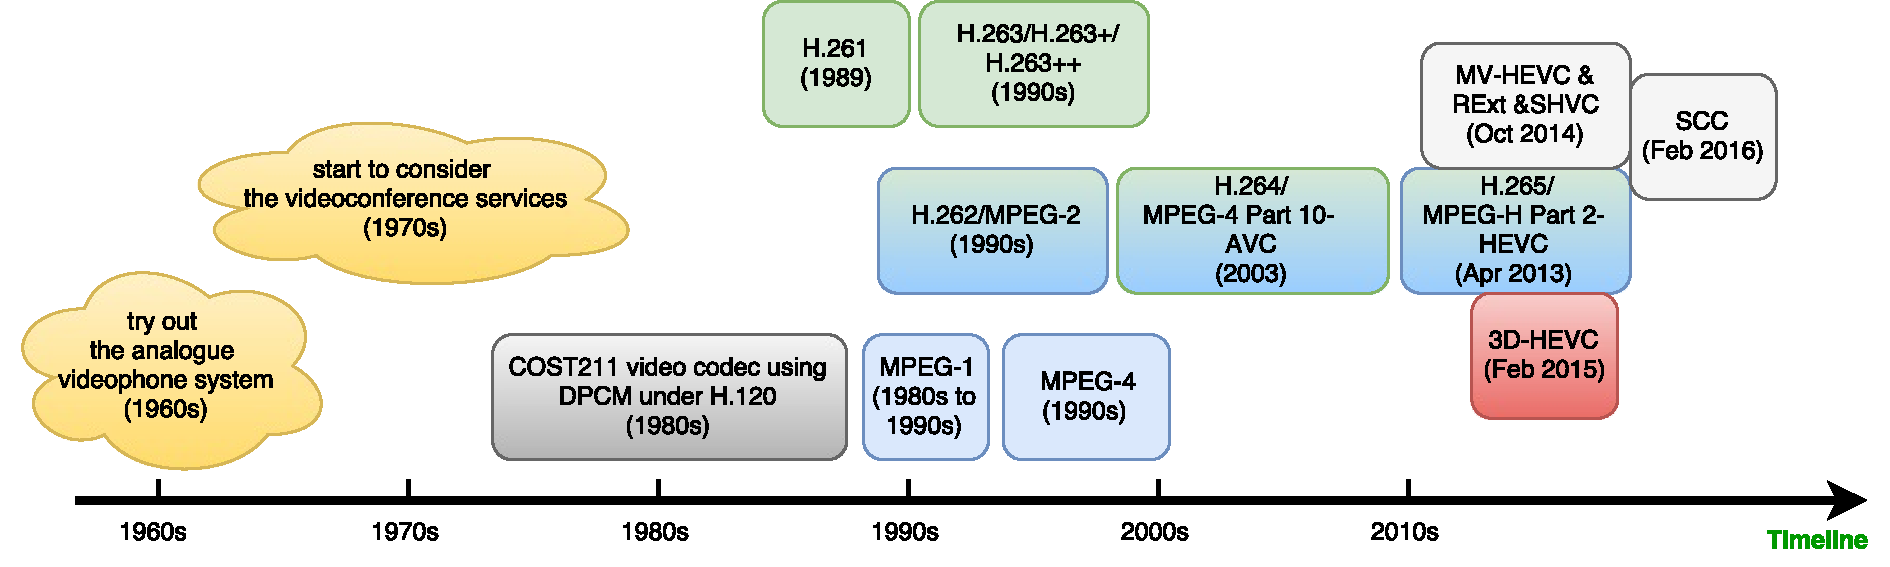
\includegraphics[width=\textwidth,height=\textheight,keepaspectratio]{Figures/video-std-brief-history.pdf}
%        \decoRule
    \caption[The brief history of the video coding standards]
    {The brief history of the video coding standards}
    \label{fig:video-std-brief-history}
\end{figure}
In 1980s, the COST211 video codec, built on top of Differential
Pulse Code Modulation (DPCM), was standardized under H.120 standard by CCITT
(now known as ITU-T).
In late 1989, the H.261 was completed and its success marked a milestone for
video coding at low bit rate with fairly good quality~\parencite{RN181}.
The Motion Picture Experts Group (MPEG) kicked off the exploration of video
storage, such as CD-ROMs.
Their objective was to achieve a competitive performance with cassette
recorders in terms of compression of videos which have rich motions.
The framework of H.261 had been used to start the codec design of MPEG-1.
MPEG-2 was one generation after the MPEG-1.
It featured higher capabilities when handling videos with
high bit rates and high resolutions.
In MPEG-2, the encoder is allowed to make its own decision on the
the number of bi-directionally predicted pictures according to a
suitable coding delay.
ITU-T found this technique applicable to telecommunication applications, as
a result MPEG-2 has been adopted as H.262 for telecommunications.
Right after the MPEG-2 standard, MPEG-3 was designed mainly for coding of
high definition videos.
However, MPEG-3 was discarded due to the versatility of MPEG-2, which
can be used to encode videos of any resolutions.
In the late 1998, MPEG-4 was introduced as a way of defining compression of
both audio and visual digital data.
Later on MPEG-4 was divided into several parts during its continuously evolving.
Among its sub-parts, MPEG-4 part 10 (a.k.a. Advanced Video Coding) is mainly
for the video compression.
With the rising popularity of the high definition videos, the new standard
termed High Efficiency Video Coding (HEVC) for compressing videos in a more
efficient way comparing with previous standards, such as H.264/AVC, has
emerged under the efforts from the Joint Collaborative Team on Video
Coding (JCT-VC).
In the meanwhile, five extensions of the HEVC standard, comprising
Format Range Extension (RExt), Scalability Extension (SHVC),
Multi-view Extension (MV-HEVC), 3D Extension (3D-HEVC),
Screen Content Coding Extension (SCC),  have been finalized
from 2014 to 2016 to fulfill extra requirements in various video coding
scenarios.

In this work, we focus on the depth map coding in 3D-HEVC\@.
The 35 angular modes and depth modeling modes have been embraced in the
depth map coding tools in 3D-HEVC\@.
The DMM1 mode introduces an huge increase for the encoding time of 3D videos.
Acceleration of the depth map coding is needed.

\section{Deep Learning}\label{sec:deep-learning}
Deep learning is an approach of representation learning
(a.k.a. feature learning), which is essentially a method to
learn from data.
Numerous layers of computational units together with appropriate activating
mechanism comprise the basic architecture for deep learning.
Multitudinous data sets are needed for those computational architectures
to learn data abstractions
for tasks such as image classification, speech recognition,
object detection, etc.
Each layer learns a level of abstraction from the data sets using
back-propagation algorithm~\parencite{RN96}.
Making use of those learned abstractions, the computational architectures are
able to solve complex problems which are typically non-linear and normally hard
to solve by using specific rules that are designed in advance.

Deep learning has been attracting wide attention from all over the world
in recent years, not only because of the great achievements it has
made in various application scenarios, but also due to the promise of an
intelligent future it gives.
Such a learning methodology makes people believe it is possible
for the formation of wise machines
that they have long dreamed to possess.
The growing data accessibility provides rich examples for deep computational
architectures to adjust their internal weights and bias until their
predictions have low error rate.
On the other hand, the computational devices are relatively
affordable than in the previous years by the society, with the help of which,
accelerations of learning processes has been achieved, hence a bunch of
time consuming deep learning architectures can be tried within acceptable
periods.

In the ILSVRC-2012 competition~\parencite{RN205}, AlexNet~\parencite{RN65}
received the championship with the 15.3\% top-5 error rate, compared to
26.2\% achieved by the runner-up.
Such a large margin of error rate claimed a breakthrough in
object recognition history.
It kicked off a blistering pace of trying out deep learning by both academia
and industry, which in turn led to an increase of the convolutional
neural networks' submissions to ILSVRC-2013, in which ZF Net~\parencite{RN66}
was the winner.
It fine-turned the architecture of AlexNet based on the
gorgeous visualizations of trained models.
Both AlexNet and ZF Net are of the same structure which is built up
by simply stacking computational layers while GoogLeNet~\parencite{RN60}
is composed of Inception
modules.
This new architecture was the most successful candidate in ILSVRC-2014.
It has not only set the new height of object recognition but also started to
optimize the computational resources of the network by design.
It consists of 22 layers, which was deeper than all the previous
networks in ILSVRC\@.
However, it is still not deep enough.
In ILSVRC-2015, Residual Neural Network (ResNet)~\parencite{RN67} with
152 layers won the championships in all the five main tracks.
ResNet introduced a brand new notion into the neural network architecture
named identity mapping.
The shortcut connection in the identity mapping prevents the degradation of
training accuracy when the network goes deeper.
Besides, the converging speed of ResNet is faster than the network built up
with Inception modules when both are of the similar size.

Despite the fact that neural networks built up from Inception modules
converge slower than those built up from ResNet modules, it is still
worth it for a brief review of the valuable insights residing in
the Inception networks.
A typical incarnation of the first generation of Inception networks is named
GoogLeNet~\parencite{RN60}.
It was intricately carved with a responsibility to win computer vision
tasks in ILSVRC-2014, on which it performed better than all the other
deep neural network architectures.
There exist philosophical reflections which are intend to serve as guidelines
for the construction of Inception networks.
Two major downsides of a enlarged neural network have been discussed
in~\parencite{RN60}.
One is the higher chances of overfitting while the other is
the strikingly increased requirements of computational resources with the
enlarged network size.
For handling those drawbacks, based on the new ideas which were introduced
in~\parencite{RN207} about how to construct the reasonable architecture of
neural networks, new experiments orienting sparse network structure have
been tried out.
One year later after GoogleNet hold the championship of ILSVRC-2014,
a method named Batch Normalization~\parencite{RN61} has been
proposed by Google researchers to accelerate and ease the
training of deep neural networks.
The core idea behind Batch Normalization is to normalize
the inputs to each layer for every batch of training data.
More importantly, based on the observation that the normalization process
essentially is matrix multiplications followed by adding biases, the Batch
Normalization is implemented as additional layers which makes it part of
the network architecture.
This fairly novel method started a new chapter for the training of deep
neural networks.
With the adoption of Batch Normalization, higher learning rates no longer
impede the convergence of the deep networks, oppositely faster
training speed is brought to scene which can achieve a
better accuracy of prediction with considerably less time.
Additionally, in some cases, it can even replace the Dropout~\parencite{RN70}
which is an effective method to prevent overfitting.
The incorporation of Batch Normalization into the first generation of
Inception network architecture led to the formation of Inception-v2, which
improved the best accuracy on ImageNet classification with less training steps.
%more advanced accuracy on ILSVRC 2012
%classification challenge validation set.
In the same year, Inception-v3~\parencite{RN62} joined the show, the objective of which was
to effectively leverage the power of additional computation by factorizing
to smaller size convolutions and regularizing the classifier layer with
the estimation of minor effect of label-dropout in the training process.
The network architectures were scaled up in Inception-v3, which consequently
imposed higher requirements of available computational resources.

% ====== can be used for literature review =====
%AlexNet contains five convolutional layers and three fully-connected
%layers.
%The Rectified Linear Units (ReLU)~\parencite{RN206}, Local Response
%Normalization and Overlapping Pooling were adopted.
%The methodology of multiple GPU training was used to make the learning fast.
%Data Augmentation and Dropout were chosen to overcome the problem of
%Overfitting.
%Stochastic gradient descent was adopted.
% ====== can be used for literature review =====




%Welcome to this \LaTeX{} Thesis Template, a beautiful and easy to use template for writing a thesis using the \LaTeX{} typesetting system.
%
%If you are writing a thesis (or will be in the future) and its subject is technical or mathematical (though it doesn't have to be), then creating it in \LaTeX{} is highly recommended as a way to make sure you can just get down to the essential writing without having to worry over formatting or wasting time arguing with your word processor.
%
%\LaTeX{} is easily able to~\parencite{RN93} professionally typeset documents that run to hundreds or thousands of pages long. With simple mark-up commands, it automatically sets out the table of contents, margins, page headers and footers and keeps the formatting consistent and beautiful. One of its main strengths is the way it can easily typeset mathematics, even \emph{heavy} mathematics. Even if those equations are the most horribly twisted and most difficult mathematical problems that can only be solved on a super-computer, you can at least count on \LaTeX{} to make them look stunning.
%
%%----------------------------------------------------------------------------------------
%
%\section{Welcome and Thanku}\label{sec:welome}
%Welcome to this \LaTeX{} Thesis Template, a beautiful and easy to use template for writing a thesis using the \LaTeX{} typesetting system.
%
%If you are writing a thesis (or will be in the future) and its subject is technical or mathematical (though it doesn't have to be), then creating it in \LaTeX{} is highly recommended as a way to make sure you can just get down to the essential writing without having to worry over formatting or wasting time arguing with your word processor.
%
%\LaTeX{} is easily able to professionally typeset documents that run to hundreds or thousands of pages long. With simple mark-up commands, it automatically sets out the table of contents, margins, page headers and footers and keeps the formatting consistent and beautiful. One of its main strengths is the way it can easily typeset mathematics, even \emph{heavy} mathematics. Even if those equations are the most horribly twisted and most difficult mathematical problems that can only be solved on a super-computer, you can at least count on \LaTeX{} to make them look stunning.
%
%%----------------------------------------------------------------------------------------
%
%\section{Welcome and ThYou}\label{sec:weome}
%Welcome to this \LaTeX{} Thesis Template~\parencite{Reference1}, a beautiful and easy to use template for writing a thesis using the \LaTeX{} typesetting system.
%
%If you are writing a thesis (or will be in the future) and its subject is technical or mathematical (though it doesn't have to be), then creating it in \LaTeX{} is highly recommended as a way to make sure you can just get down to the essential writing without having to worry over formatting or wasting time arguing with your word processor.
%
%\LaTeX{} is easily able to professionally typeset documents that run to hundreds or thousands of pages long. With simple mark-up commands, it automatically sets out the table of contents, margins, page headers and footers and keeps the formatting consistent and beautiful. One of its main strengths is the way it can easily typeset mathematics, even \emph{heavy} mathematics. Even if those equations are the most horribly twisted and most difficult mathematical problems that can only be solved on a super-computer, you can at least count on \LaTeX{} to make them look stunning.
%
%%----------------------------------------------------------------------------------------
%
%\section{Welcome and Thau}\label{sec:welcoe}
%Welcome to this \LaTeX{} Thesis Template, a beautiful and easy to use template for writing a thesis using the \LaTeX{} typesetting system.
%
%If you are
%\begin{table}
%
%    \label{tab:treatments}
%    \centering
%%    \begin{tabular}{l l l}
%%        \toprule
%%        \tabhead{Groups} & \tabhead{Treatment X} & \tabhead{Treatment Y} \\
%%        \midrule
%%        1 & 0.2 & 0.8\\
%%        2 & 0.17 & 0.7\\
%%        3 & 0.24 & 0.75\\
%%        4 & 0.68 & 0.3\\
%%        \bottomrule\\
%%    \end{tabular}
%    \begin{tabular}{c r @{.} l}
%        Pi expression       &
%        \multicolumn{2}{c}{Value} \\
%        \hline
%        $\pi$               & 3&1416  \\
%        $\pi^{\pi}$         & 36&46   \\
%        $(\pi^{\pi})^{\pi}$ & 80662&7 \\
%    \end{tabular}
%    \caption{The effects of treatments X and Y on the four groups studied.}
%\end{table}
%writing a thesis (or will be in the future) and its subject is technical or mathematical (though it doesn't have to be), then creating it in \LaTeX{} is highly recommended as a way to make sure you can just get down to the essential writing without having to worry over formatting or wasting time arguing with your word processor.
%
%\LaTeX{} is easily able to professionally typeset documents that run to hundreds or thousands of pages long. With simple mark-up commands, it automatically sets out the table of contents, margins, page headers and footers and keeps the formatting consistent and beautiful. One of its main strengths is the way it can easily typeset mathematics, even \emph{heavy} mathematics. Even if those equations are the most horribly twisted and most difficult mathematical problems that can only be solved on a super-computer, you can at least count on \LaTeX{} to make them look stunning.
%
%%----------------------------------------------------------------------------------------
%
%\section{Welcome and Tnk You}\label{sec:wlcome}
%Welcome to this \LaTeX{} Thesis Template, a beautiful and easy to use template for writing a thesis using the \LaTeX{} typesetting system.
%
%If you are writing a thesis.
%
%%\begin{verbatim}
%\begin{figure}
%    \centering
%    
\includegraphics{Figures/Electron}
%    %    \decoRule
%    \caption[An Electron]{An electron (artist's impression).}
%    \label{fig:Electron}
%\end{figure}
%%\end{verbatim}
%(or will be in the future) and its subject is technical or mathematical (though it doesn't have to be), then creating it in \LaTeX{} is highly recommended as a way to make sure you can just get down to the essential writing without having to worry over formatting or wasting time arguing with your word processor.
%
%\LaTeX{} is easily able to professionally typeset documents that run to hundreds or thousands of pages long. With simple mark-up commands, it automatically sets out the table of contents, margins, page headers and footers and keeps the formatting consistent and beautiful. One of its main strengths is the way it can easily typeset mathematics, even \emph{heavy} mathematics. Even if those equations are the most horribly twisted and most difficult mathematical problems that can only be solved on a super-computer, you can at least count on \LaTeX{} to make them look stunning.
%
%%----------------------------------------------------------------------------------------